\documentclass[xcolor=dvipsnames]{beamer}
\usepackage[T1]{fontenc}
\usepackage[utf8]{inputenc}
\usepackage[english,slovak]{babel}

\usepackage{amsmath}
\usepackage{amsthm}
\usetheme{Pittsburgh}
\useoutertheme{shadow}

\usepackage{graphicx}
\usepackage{caption}
\usepackage{subcaption}

\usepackage[]{algorithm2e}
\usepackage{listings}
 \setbeamercovered{transparent}
 \usepackage{cuted}
\usepackage[export]{adjustbox}
\usepackage{mathtools}

\usepackage{lipsum}
\usepackage{verbatim}
\usepackage{transparent}
\usepackage{framed}
\usepackage{xcolor}

\usepackage{multirow}
\usepackage{colortbl}
\usepackage{lmodern}

\usepackage{movie15}
\usepackage{media9}
\usepackage{verbatim}

\usepackage{hyperref}

\usepackage{movie15}

\newcommand\Wider[2][3em]{%
\makebox[\linewidth][c]{%
  \begin{minipage}{\dimexpr\textwidth+#1\relax}
  \raggedright#2
  \end{minipage}%
  }%
}






\iftrue

\usetheme{Warsaw}

\setbeamercolor{normal text}{fg=white,bg=black!90}
\setbeamercolor{structure}{fg=white}

\setbeamercolor{alerted text}{fg=red!85!black}

\setbeamercolor{item projected}{use=item,fg=black,bg=item.fg!35}

\setbeamercolor*{palette primary}{use=structure,fg=structure.fg}
\setbeamercolor*{palette secondary}{use=structure,fg=structure.fg!95!black}
\setbeamercolor*{palette tertiary}{use=structure,fg=structure.fg!90!black}
\setbeamercolor*{palette quaternary}{use=structure,fg=structure.fg!95!black,bg=black!80}

\setbeamercolor*{framesubtitle}{fg=white}

\setbeamercolor*{block title}{parent=structure,bg=black!60}
\setbeamercolor*{block body}{fg=black,bg=black!10}
\setbeamercolor*{block title alerted}{parent=alerted text,bg=black!15}
\setbeamercolor*{block title example}{parent=example text,bg=black!15}

\fi



%-------------------------------------------------------------------------------------
\title{\color{white} \bf DQN}
\author{\color{white} Michal CHOVANEC, PhD}


%\setbeamertemplate{footline}[frame number]{}
\setbeamertemplate{navigation symbols}{}


\date[EURP]{}
\begin{document}



{
    \usebackgroundtemplate
    {
        \vbox to \paperheight{\vfil\hbox to \paperwidth{\hfil

        {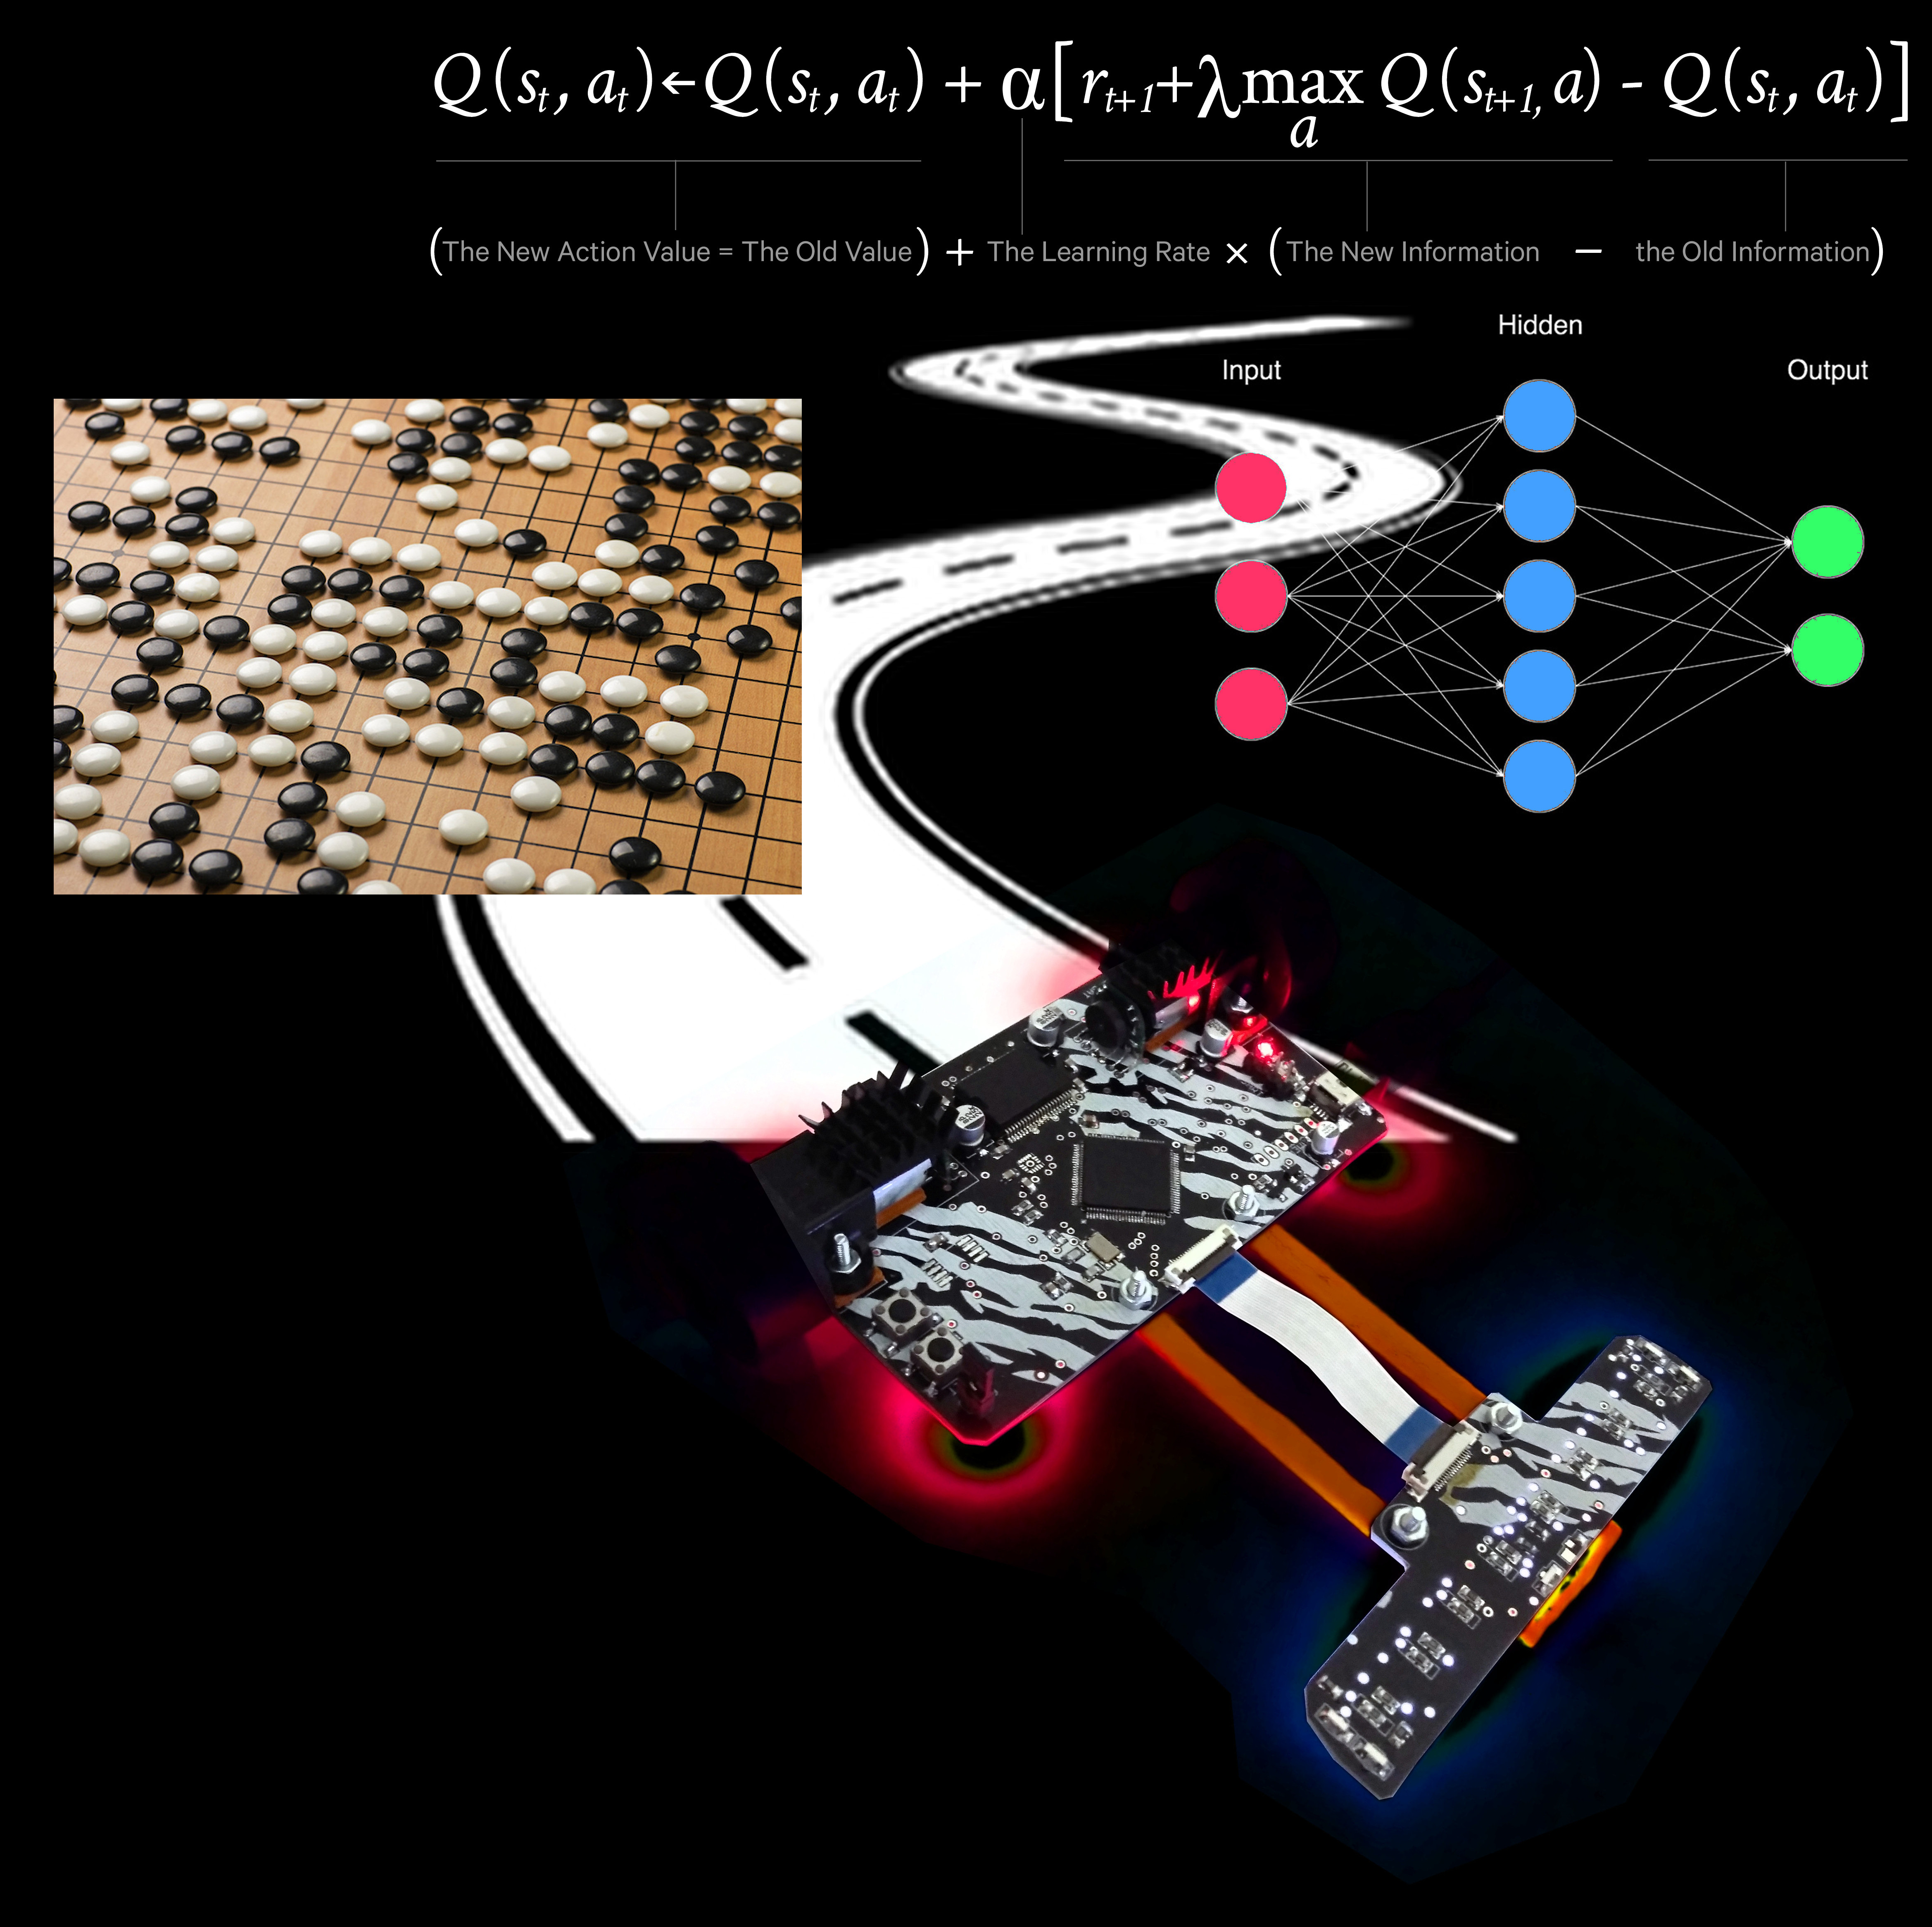
\includegraphics[width=5.05in]{./pictures/rl_square.jpg}}

        \hfil}\vfil}
    }



    \begin{frame}

    \centering
     \colorbox{black}
     {
        \begin{minipage}{7cm}
           {\LARGE \color{white} \bf reinforcement learning} \\
           {\LARGE \color{white} Michal CHOVANEC} \\
       \end{minipage}
     }

    \end{frame}
}

\begin{frame}{\bf reinforcement learning}

\begin{columns}
  \begin{column}{0.5\textwidth}
      \centering
      \includemovie[
        poster,
        autoplay,
        externalviewer,
        inline=false,
        text={ 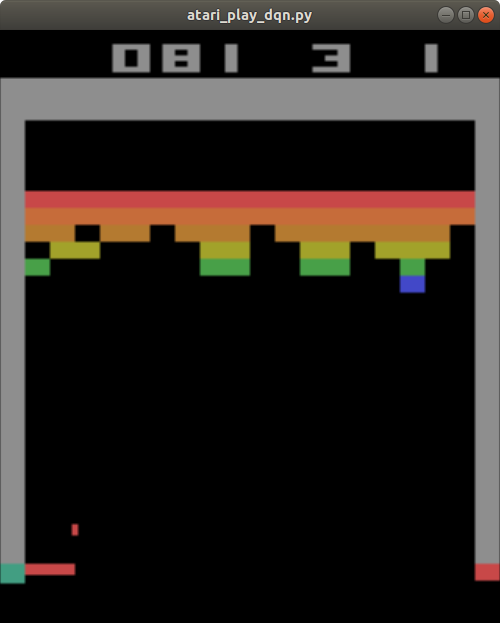
\includegraphics[scale=0.15]{./pictures/breakout.png}}
      ]{3cm}{3.3cm}{./video/rl_atari.mp4}

  \begin{figure}
    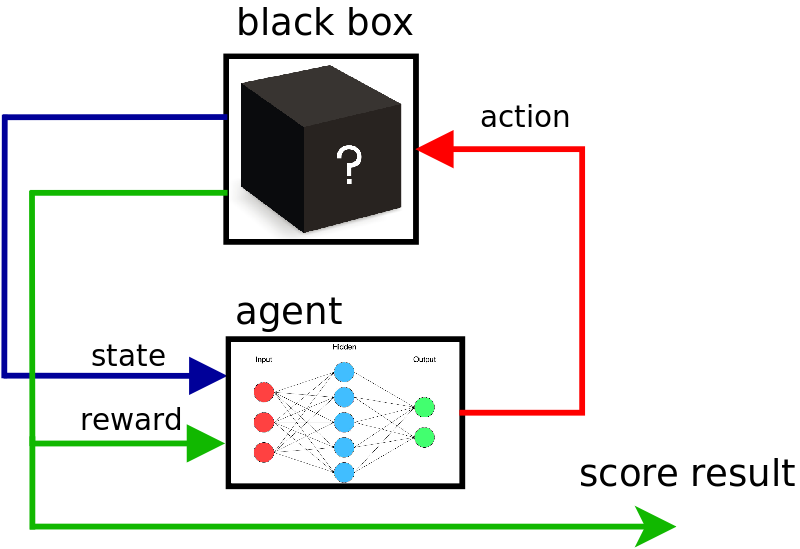
\includegraphics[scale=0.3]{./diagrams/rl_mechanism.png}
  \end{figure}

  \end{column}
  \begin{column}{0.5\textwidth}  %%<--- here

  {\bf
    \begin{itemize}
      \item learning from punishments and rewards
      \item learn to play a game with unknow rules
    \end{itemize}
  }

  \begin{enumerate}
    \item obtain {\bf state}
    \item choose {\bf action}
    \item {\bf execute} action
    \item obtain {\bf reward}
    \item learn from {\bf experiences}, $Q(s, a)$, or $\pi(a|s)$
  \end{enumerate}


  \end{column}
\end{columns}

\end{frame}


\begin{frame}{\bf intro - milestones}
   \begin{itemize}
      \item 1997 Gari Kasparov, decission trees - Deep Blue
      \item 1997 Jürgen Schmidhuber, LSTM - recurrent neural network
      \item 1998 Yann LeCun, LeNet - convolutional neural network
      \item 2012 Alex Krizhevsky, Goefrey Hinton, AlexNET - image recognition
      \item {\bf 2013 Mnih, DQN - playing Atari}
      \item {\bf 2016 DeepMind, GO - AlphaGO vs Lee Sedol}
      \item {\bf 2019 DeepMind, StarCraft - AlphaStar vs MaNa}
    \end{itemize}
\end{frame}

\begin{frame}{\bf algorithms}
   \begin{itemize}
    \item Value based

        \begin{itemize}
          \item Deep Q-network, DQN
          \item Dueling DQN
          \item Deep deterministc policy gradient
          \item D4PG, SDDPG ...
        \end{itemize}

    \item Policy based
    
        \begin{itemize}
          \item Reinforce, temporal difference
          \item Actor Critic
          \item Advantage Actor Critic
          \item Proximal policy optimization
          \item Soft Actor critic
        \end{itemize}

    \item Model based

        \begin{itemize}
          \item Curiosity
          \item World models
          \item Imagination augmented agents
        \end{itemize}
    
    \end{itemize}

\end{frame}


\begin{frame}{\bf Garri Kasparov vs Deep Blue, 1997}

\begin{columns}
  \begin{column}{0.5\textwidth}
      \centering
      {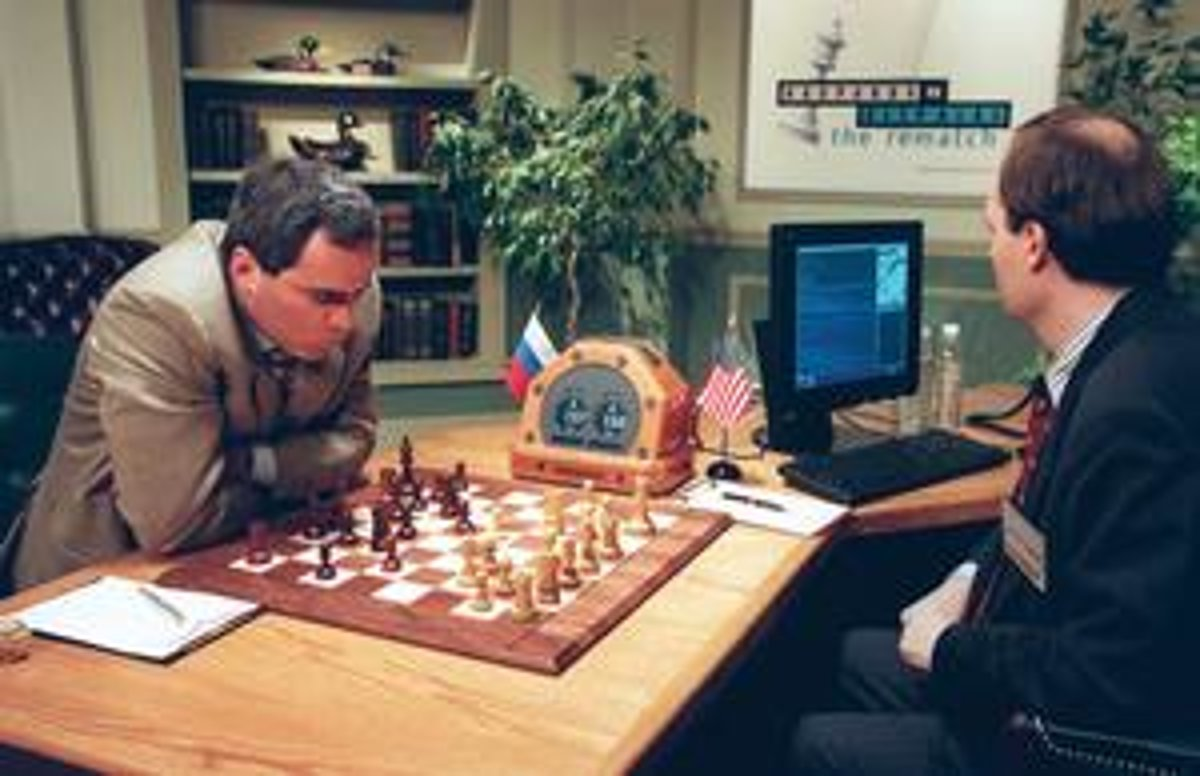
\includegraphics[width=2.05in]{./pictures/kasparov.jpg}}
  \end{column}
  \begin{column}{0.5\textwidth}  %%<--- here
      \centering
      {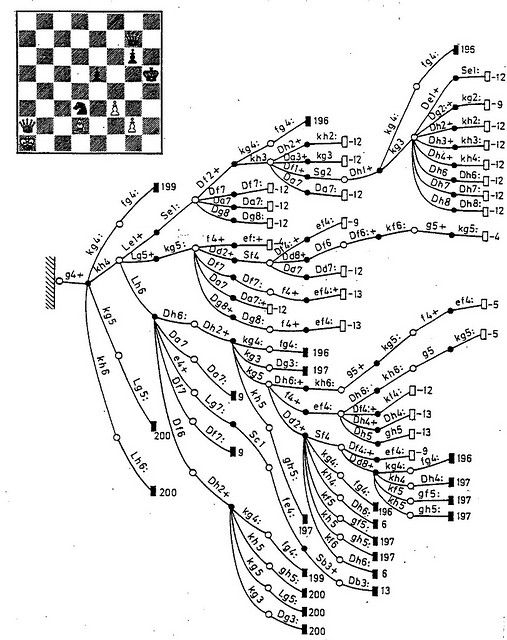
\includegraphics[width=2.05in]{./pictures/chess_tree.jpg}}
  \end{column}
\end{columns}

\end{frame}


\begin{frame}{\bf Lee Sedol vs AlphaGO, 2016}

\begin{columns}
  \begin{column}{0.5\textwidth}
      \centering
      {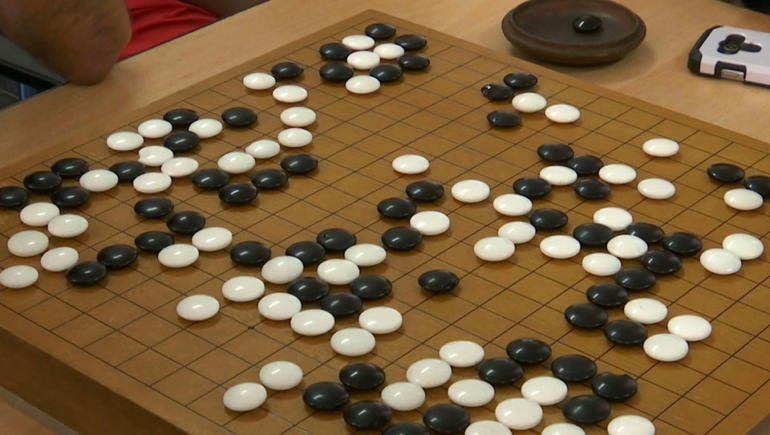
\includegraphics[width=2.05in]{./pictures/go_game.jpg}}
  \end{column}
  \begin{column}{0.5\textwidth}  %%<--- here
      \centering
      {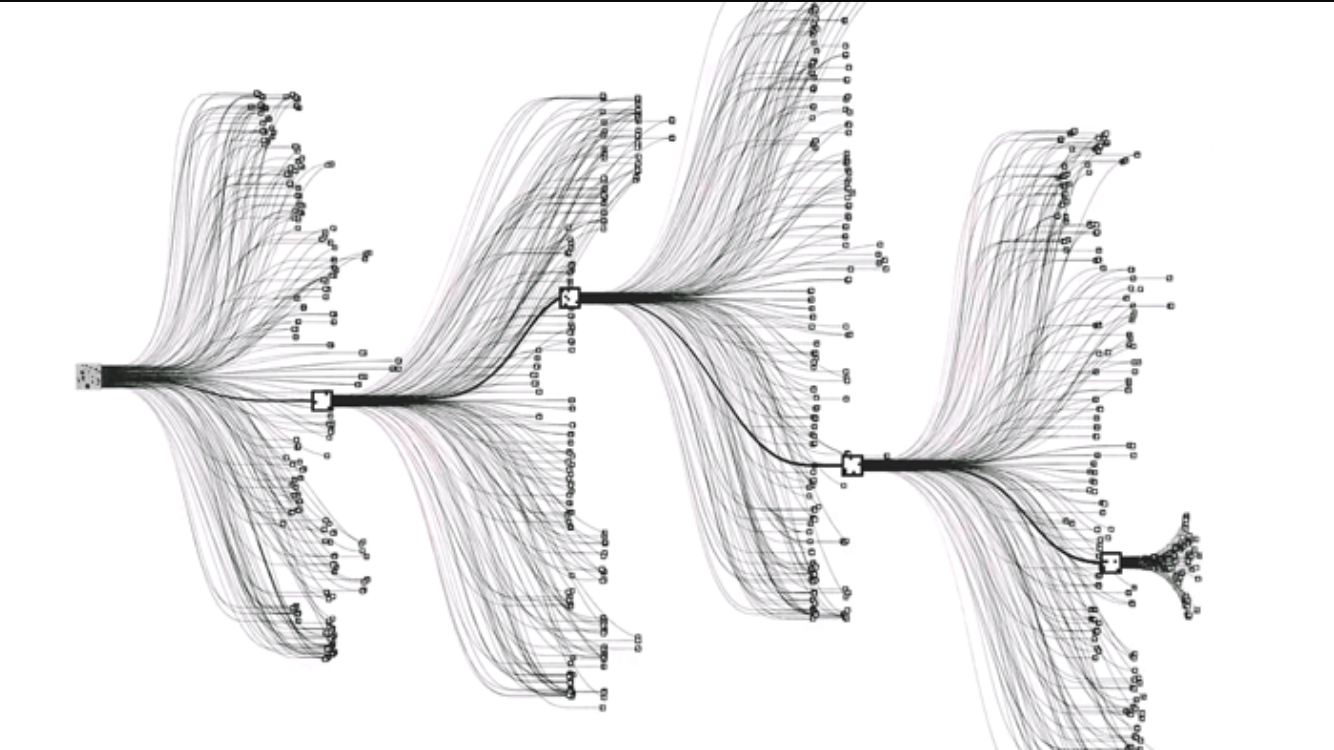
\includegraphics[width=2.05in]{./pictures/go_tree.png}}
  \end{column}
\end{columns}

\end{frame}


\begin{frame}{\bf AlphaGO}

\begin{columns}
  \begin{column}{0.5\textwidth}
      \centering
      {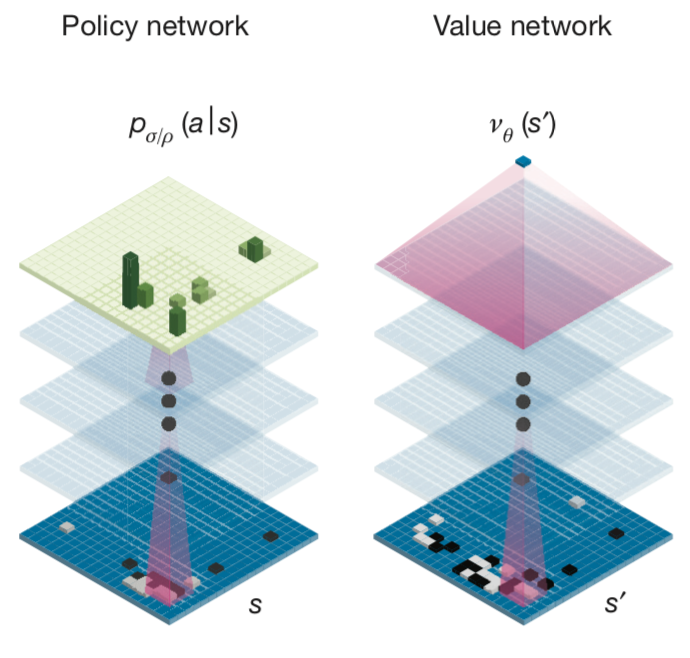
\includegraphics[width=2.05in]{./pictures/alpha_go_net.png}}
  \end{column}
  \begin{column}{0.5\textwidth}  %%<--- here
        \begin{itemize}
          \item convolutional neural networks
          \item policy net
          \item value net
        \end{itemize}  
  \end{column}
\end{columns}

\end{frame}


\begin{frame}{\bf 2048 game}

\begin{columns}
  \begin{column}{0.5\textwidth}
      \centering
      {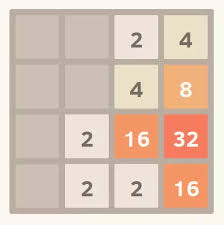
\includegraphics[width=2.05in]{./pictures/2048.jpg}}
  \end{column}
  \begin{column}{0.5\textwidth}  %%<--- here
        \begin{itemize}
          \item convolutional neural networks
          \item Q-net
        \end{itemize}  
  \end{column}
\end{columns}


{   \centering
    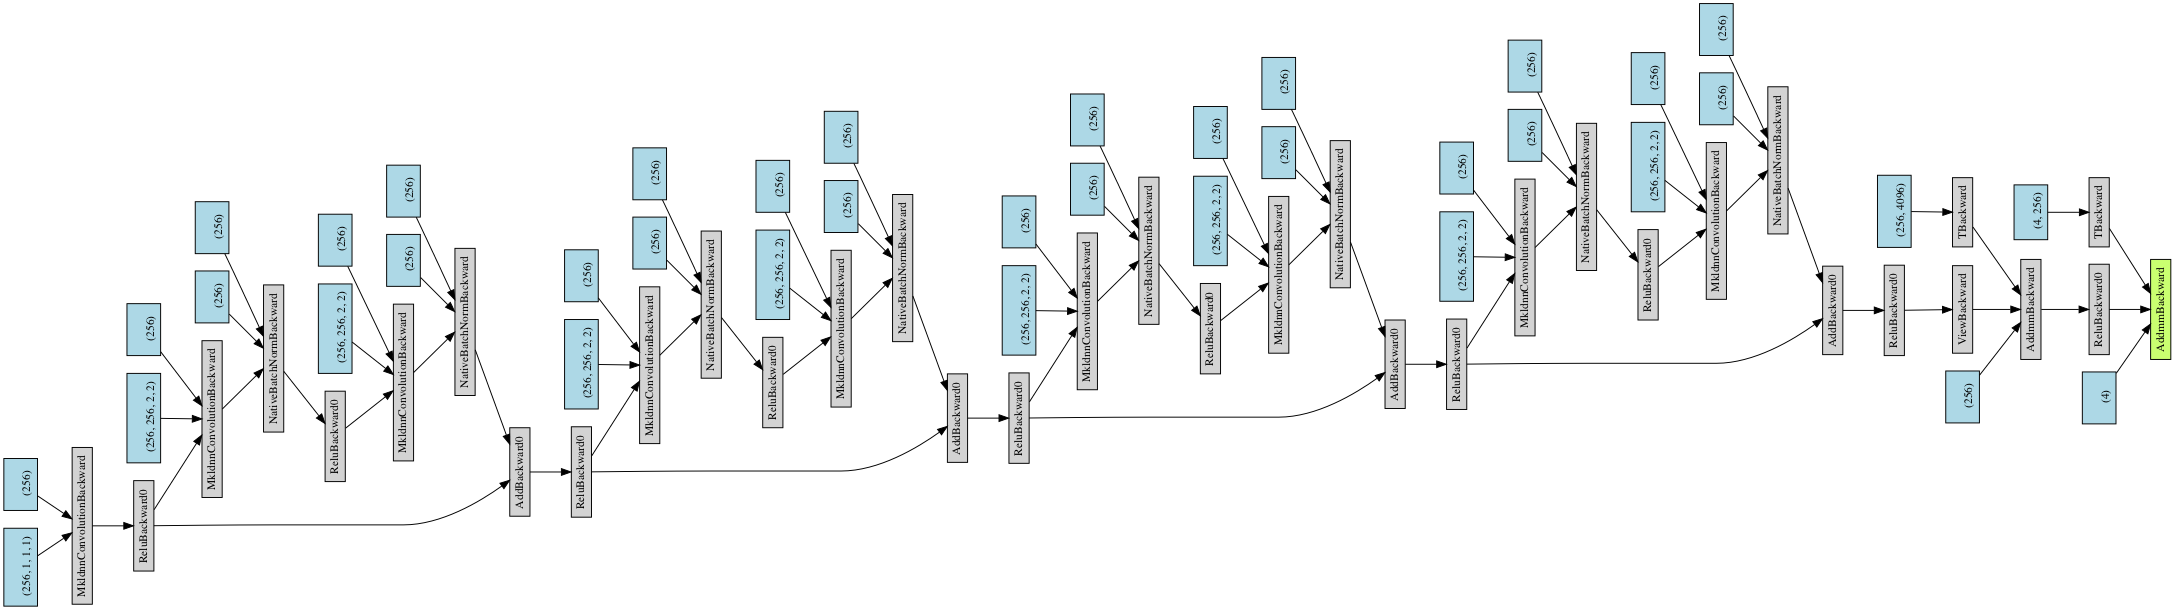
\includegraphics[width=4.0in]{./diagrams/2048_model.png}
}

\end{frame}


\begin{frame}{\bf robotics - pybullet}

\begin{columns}
  \begin{column}{0.5\textwidth}
      \centering
      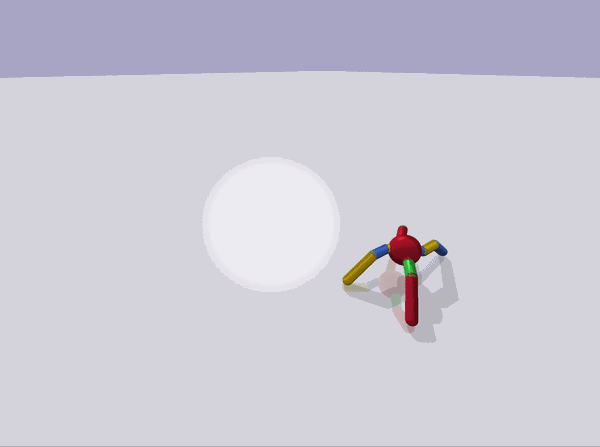
\includegraphics[width=2.0in]{./pictures/ant.png}

  \end{column}
  \begin{column}{0.5\textwidth}  %%<--- here
      \centering
      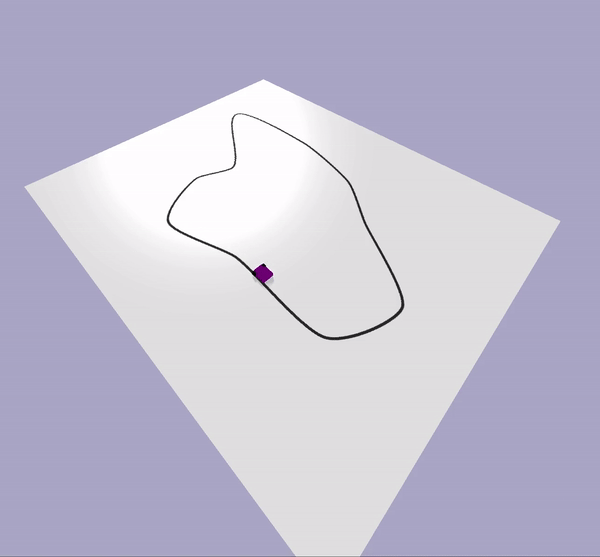
\includegraphics[width=2.0in]{./pictures/line_follower.png}
  \end{column}
\end{columns}


\end{frame}


\begin{frame}{\bf robotics - pybullet}

\begin{columns}
  \begin{column}{0.5\textwidth}
      \centering
      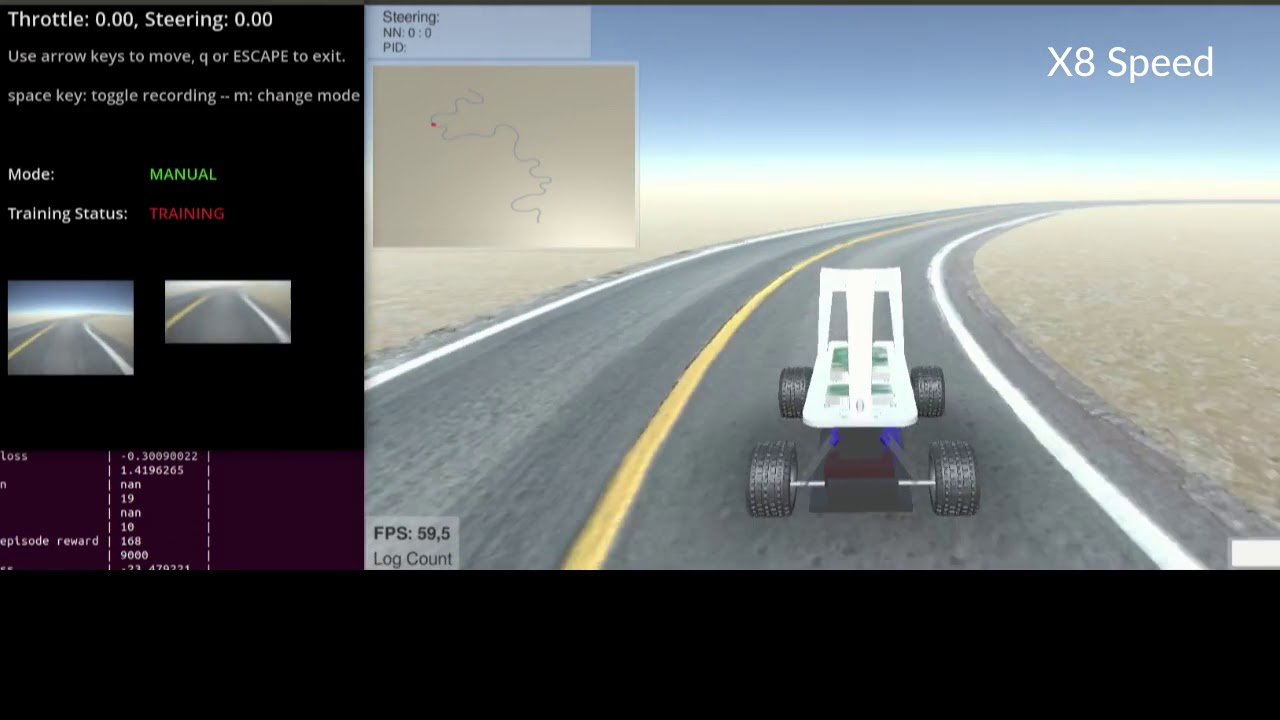
\includegraphics[width=2.5in]{./pictures/sac_car.jpg}

  \end{column}
  \begin{column}{0.5\textwidth}  %%<--- here
      \centering
      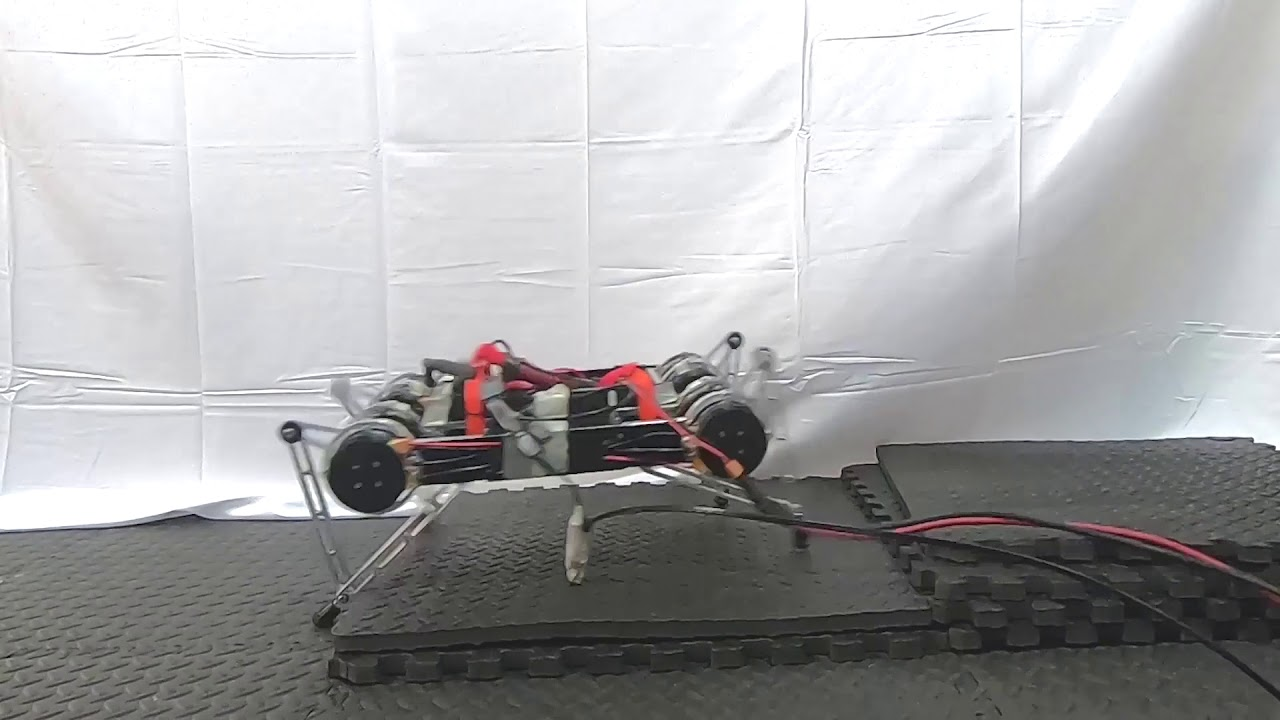
\includegraphics[width=2.5in]{./pictures/sac_minitaur.jpg}
  \end{column}
\end{columns}


\end{frame}



\begin{frame}{\bf neural networks}
  \begin{columns}
    \begin{column}{0.5\textwidth}
        \centering
        {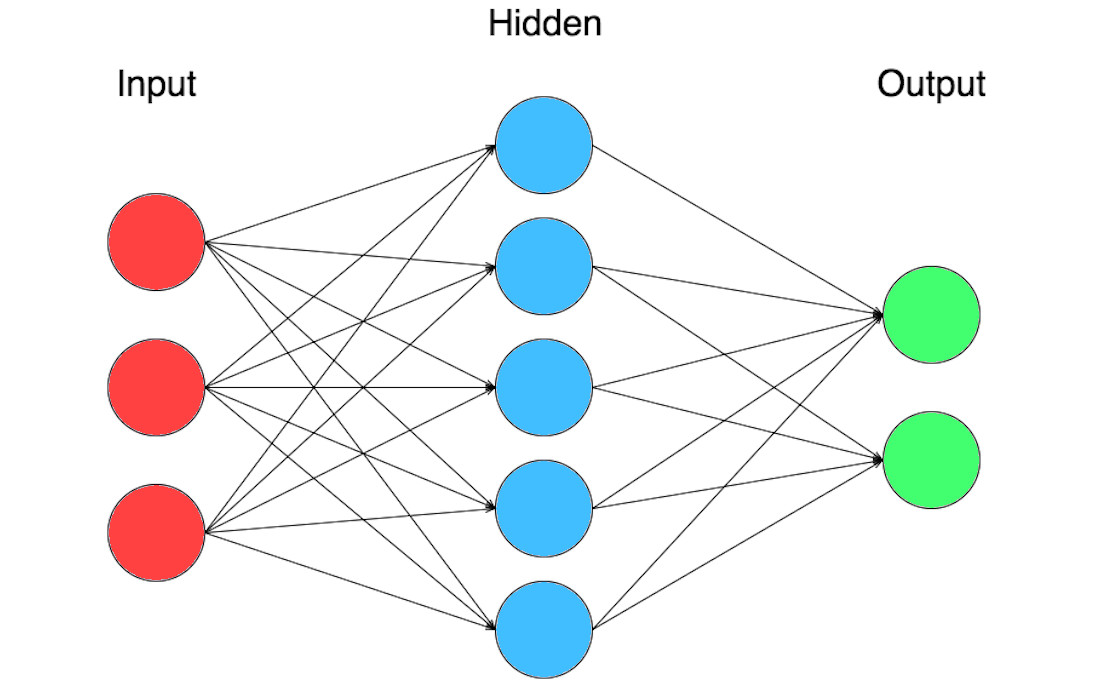
\includegraphics[width=2.05in]{./diagrams/nn.jpg}}
    \end{column}
    \begin{column}{0.5\textwidth}  %%<--- here
          \begin{itemize}
            \item requires training
            \item many layers
            \item neurons, weights
          \end{itemize}  
    \end{column}
  \end{columns}
\end{frame}


\begin{frame}{\bf deep neural networks}
  \centering
  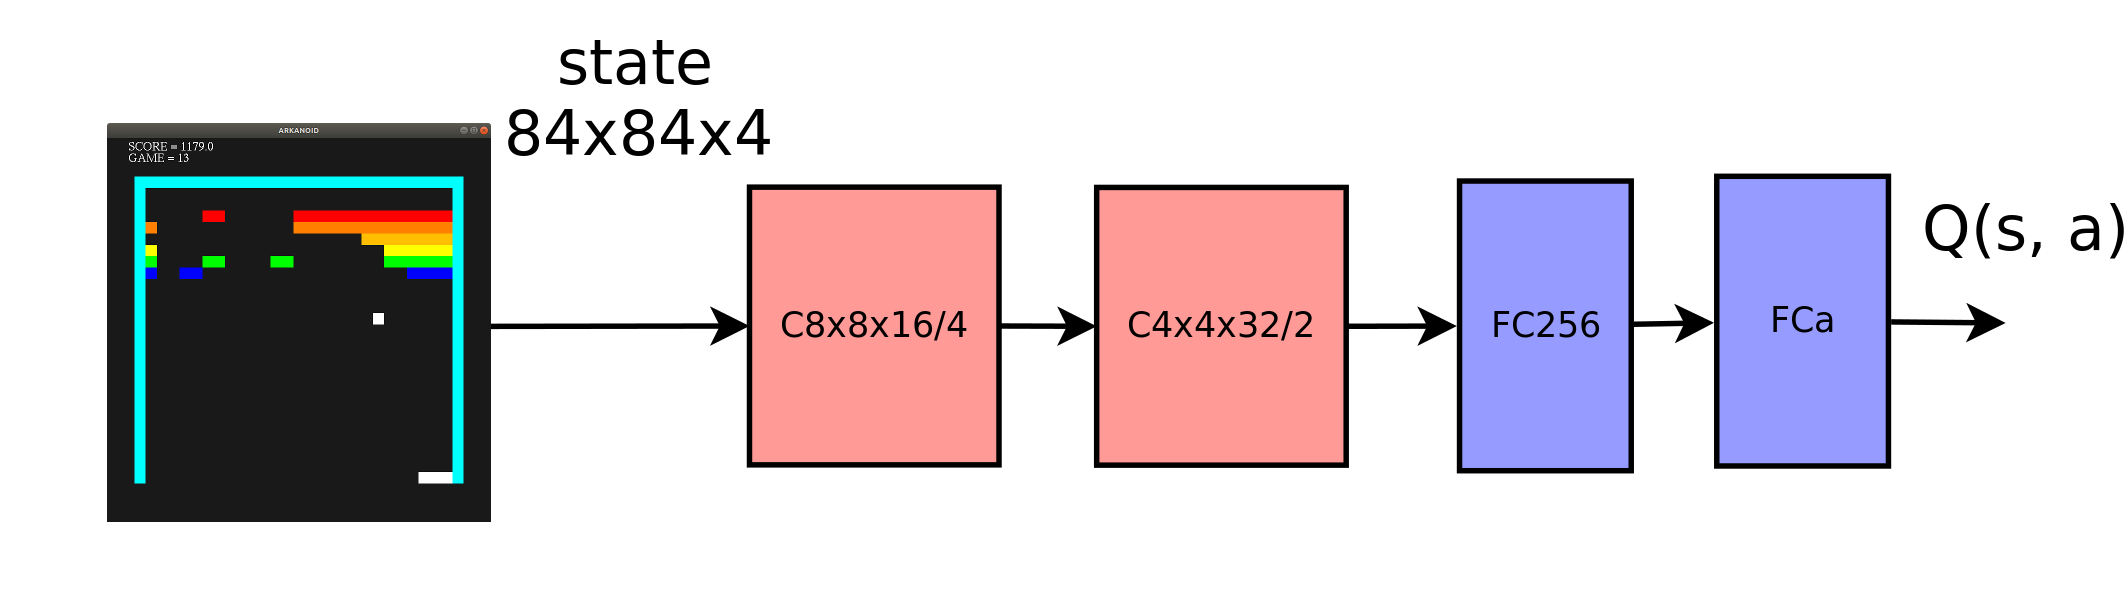
\includegraphics[width=3.05in]{./diagrams/dqn_mnih_atari.png}
  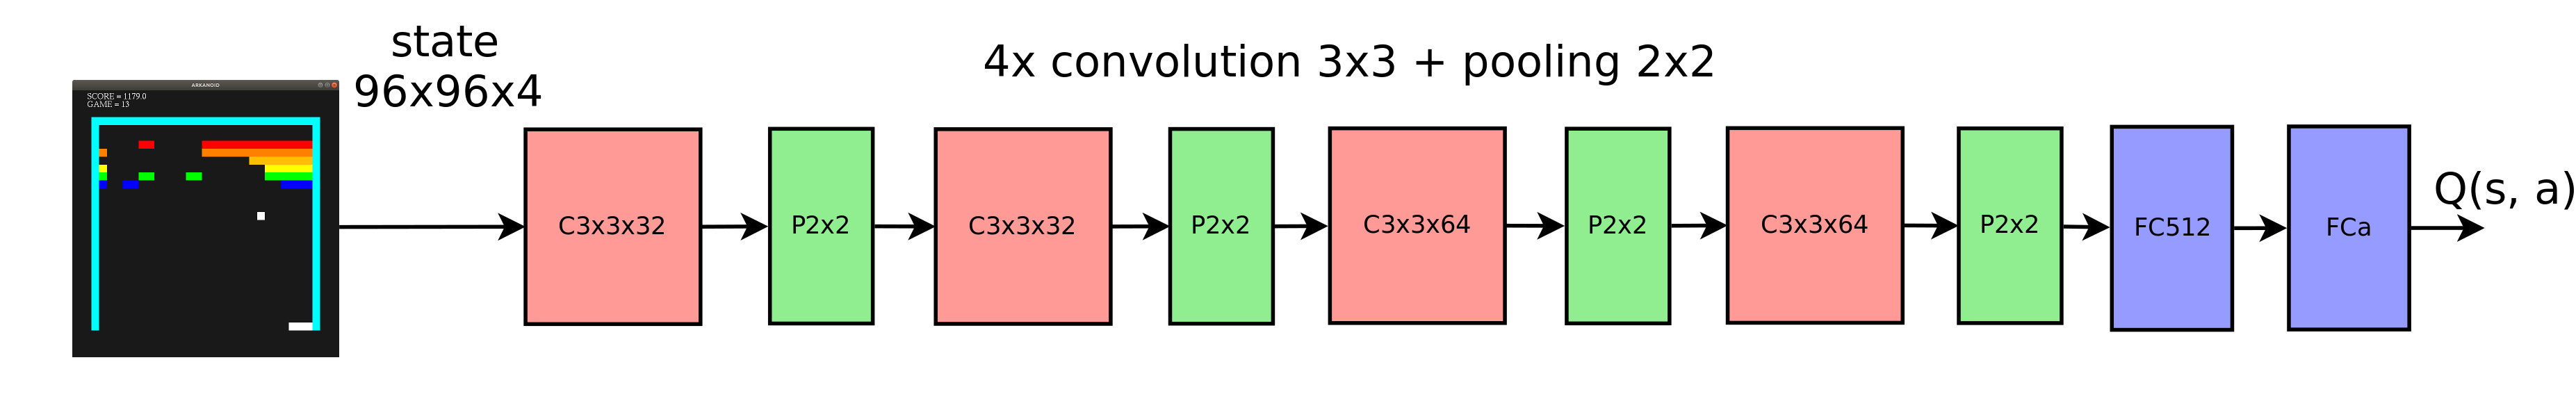
\includegraphics[width=3.05in]{./diagrams/dqn_my_atari.png}
  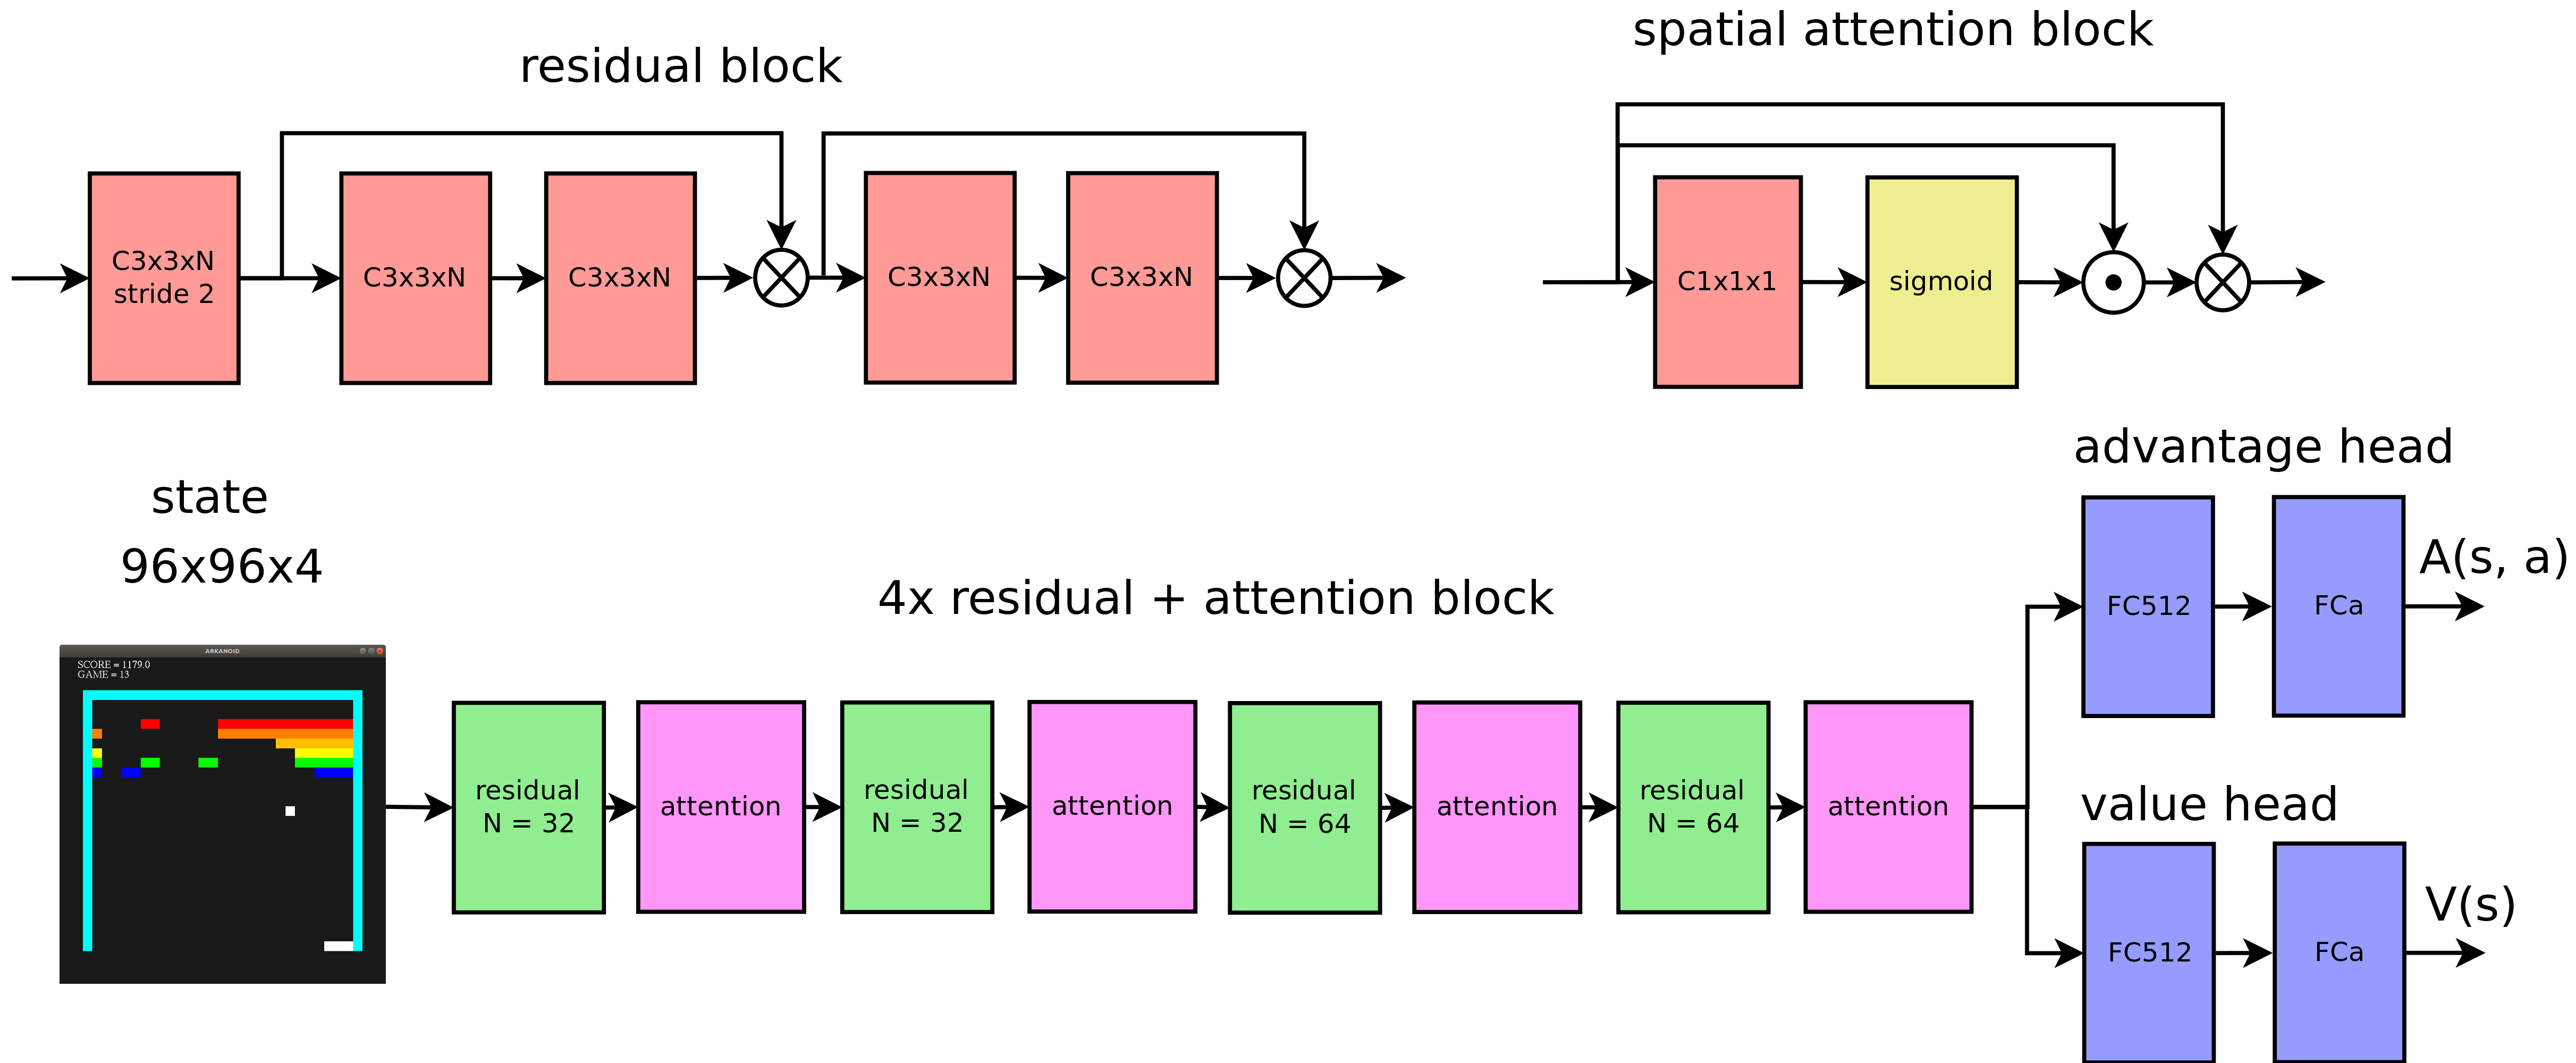
\includegraphics[width=3.05in]{./diagrams/attention_dueling_dqn_my_atari.png}

\end{frame}


\begin{frame}{\bf Q-learning}


\begin{columns}
  \begin{column}{0.5\textwidth}
    
    $Q(s, a)$ : what is the potential reward in state {\bf s} and action {\bf a}

    \begin{align*}
      Q'(s, a) = R + \gamma \max \limits_{a'} Q(s', a')
    \end{align*}

  \end{column}
  \begin{column}{0.5\textwidth}  %%<--- here

    where \\
    $s$ is state \\
    $a$ is action \\
    $s'$ is next state \\
    $a'$ is best action in next state \\
    $R$ is reward \\
    $\gamma \in \langle 0, 1 \rangle$ is discount factor \\

  \end{column}
\end{columns}

\begin{figure}
  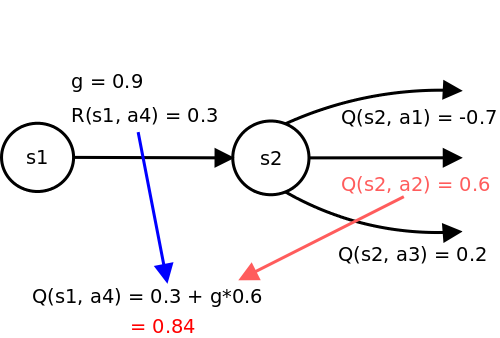
\includegraphics[scale=0.25]{diagrams/q_learning_detail.png}
\end{figure}

\end{frame}



\begin{frame}{\bf how to start}

    \begin{itemize}
      \item computer
        \begin{itemize}
          \item small models - CPU (i7, ryzen 3950x)
          \item big models - GPU (NVIDIA gtx1060)
        \end{itemize}
        \item pytorch - neural network framework
        \item pybullet - physic simulator, robotics
        \item numpy, PIL, opencv - common libs, good to know
        \item math : algebra, calculus, probaility theory, markov decision process, monte carlo integrals, diferential equations, calculus of variations
    \end{itemize}

\end{frame}

\begin{frame}{\bf hello world - lunar lander}

\begin{columns}
  \begin{column}{0.5\textwidth}
    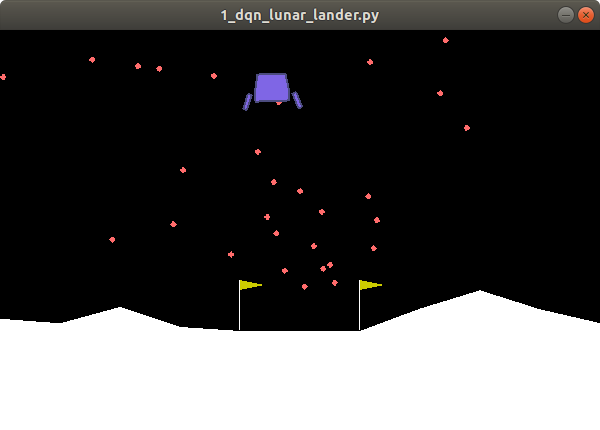
\includegraphics[scale=0.25]{./pictures/lunar_lander.png}

  \end{column}
  \begin{column}{0.5\textwidth}  %%<--- here
    \begin{itemize}
      \item discrete - three actions
        
        \begin{itemize}
          \item three actions
          \item DQN
          \item network : IN8 - FC128 - FC64 - FC3
        \end{itemize}

      \item continuous - two actions

         \begin{itemize}
          \item two actions
          \item DDPG
          \item actor network : IN8 - FC128 - FC64 - FC2
          \item critic network : IN8+2 - FC128 - FC64 - FC1
        \end{itemize}

    \end{itemize}
  \end{column}
\end{columns}


\end{frame}




\begin{frame}{\bf atari}


\begin{columns}

  \begin{column}{0.5\textwidth}
        
    \begin{figure}
      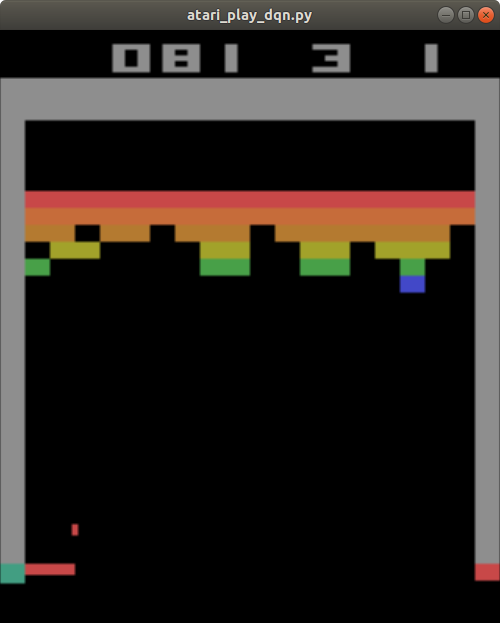
\includegraphics[scale=0.15]{./pictures/breakout.png}
    \end{figure}

  \end{column}

  \begin{column}{0.5\textwidth}
    \begin{figure}
      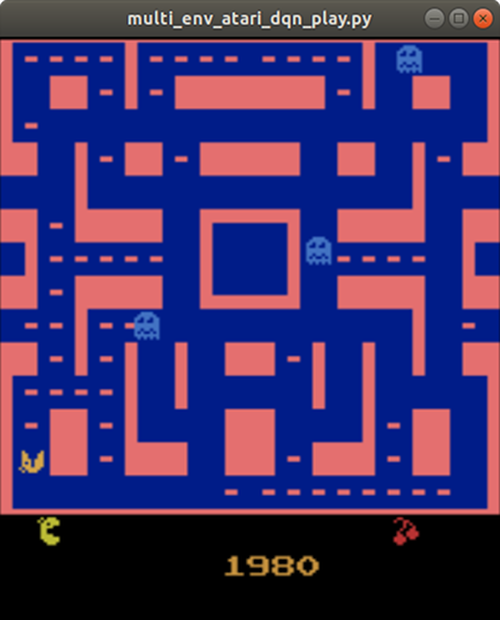
\includegraphics[scale=0.15]{./pictures/pacman.png}
    \end{figure}
  \end{column}

\end{columns}

   
\begin{columns}

  \begin{column}{0.5\textwidth}
    \begin{figure}
      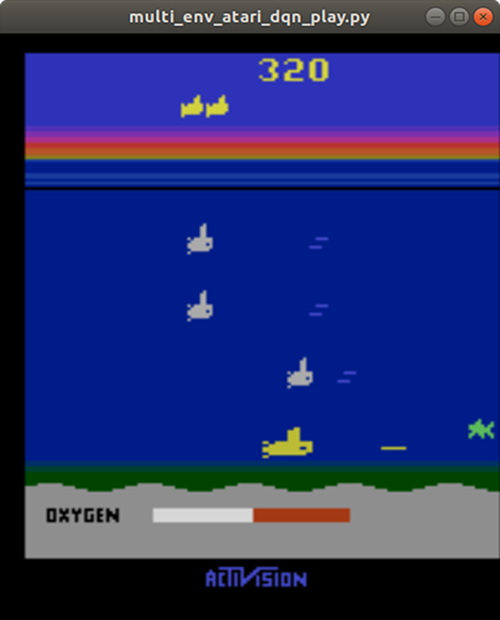
\includegraphics[scale=0.15]{./pictures/seaquest.png}
    \end{figure}
  \end{column}

  \begin{column}{0.5\textwidth}
    \begin{figure}
      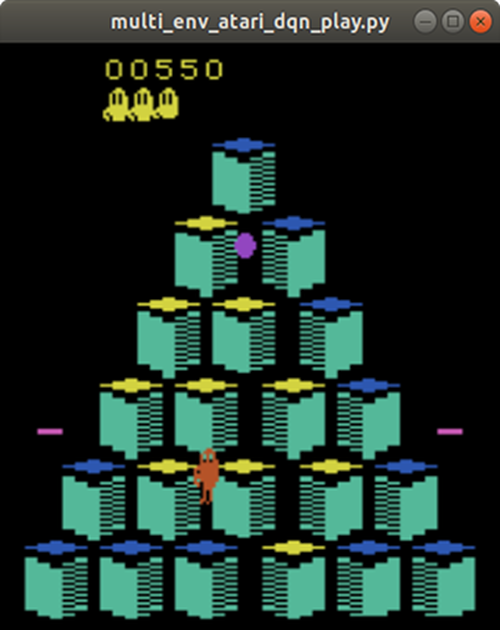
\includegraphics[scale=0.15]{./pictures/qbert.png}
    \end{figure}
  \end{column}


\end{columns}

\end{frame}







\begin{frame}{\bf where is it looking for}


\begin{columns}

  \begin{column}{0.5\textwidth}
        
    \begin{figure}
      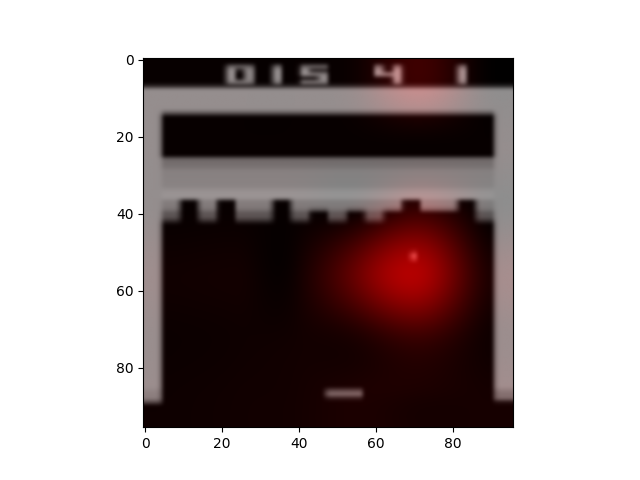
\includegraphics[scale=0.28]{./pictures/attention_breakout_dqn.png}
    \end{figure}

  \end{column}

  \begin{column}{0.5\textwidth}
    \begin{figure}
      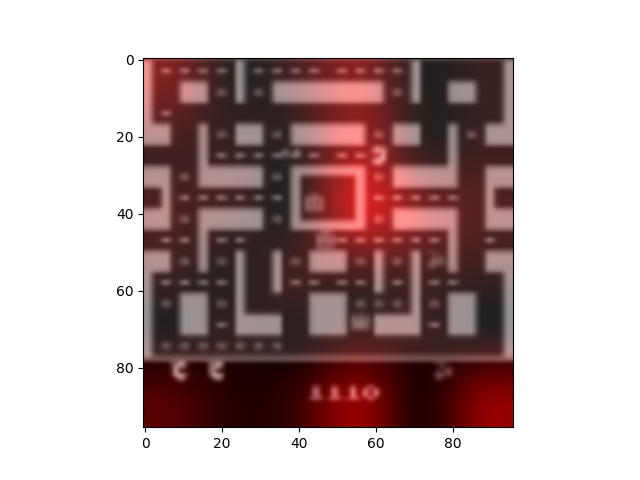
\includegraphics[scale=0.28]{./pictures/attention_pacman_dqn.png}
    \end{figure}
  \end{column}

\end{columns}

     \centering
     \includemovie[
        poster,
        autoplay,
        externalviewer,
        inline=false,
        text={video}
      ]{1cm}{0.5cm}{./video/rl_pacman.mp4}

\begin{columns}

  \begin{column}{0.5\textwidth}
    \begin{figure}
      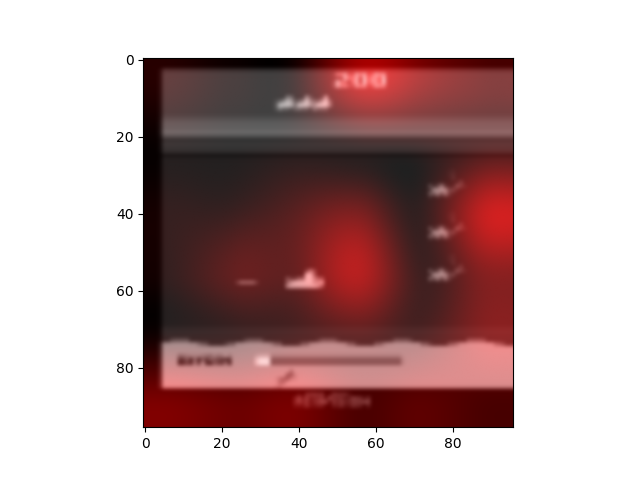
\includegraphics[scale=0.28]{./pictures/attention_seaquest_dqn.png}
    \end{figure}
  \end{column}

  \begin{column}{0.5\textwidth}
    \begin{figure}
      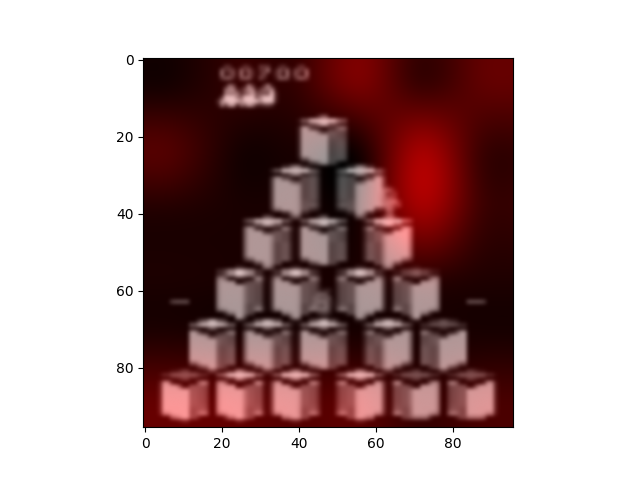
\includegraphics[scale=0.28]{./pictures/attention_qbert_dqn.png}
    \end{figure}
  \end{column}


\end{columns}

\end{frame}









\begin{frame}{\bf what is it looking for}

    \begin{figure}
      
\includegraphics[scale=0.3]{./pictures/kernel_visualisation_pacman/0.png}
    \end{figure}

    \begin{figure}
      
\includegraphics[scale=0.3]{./pictures/kernel_visualisation_pacman/3.png}
    \end{figure}


\end{frame}


\begin{frame}{\bf what is it looking for}

    \begin{figure}
      
\includegraphics[scale=0.3]{./pictures/kernel_visualisation_pacman/6.png}
    \end{figure}

\end{frame}





\begin{frame}{\bf books to read}

\begin{itemize}
  \item Maxim Lapan, 2018, Deep Reinforcement Learning Hands-On
  \item Praveen Palanisamy, 2018, Hands-On Intelligent Agents with OpenAI Gym
  \item Andrea Lonza, 2019, Reinforcement Learning Algorithms with Python
  \item Rajalingappaa Shanmugamani, 2019, Python Reinforcement Learning
  \item Micheal Lanham, 2019, Hands-On Deep Learning for Games

\end{itemize}

{\bf
  \begin{itemize}
    \item mail michal.nand@gmail.com
    \item github \href{https://github.com/michalnand/}{https://github.com/michalnand/}
    \item RL tutorial \href{https://github.com/michalnand/reinforcement_learning_tutorial}{RL tutorial {\small https://github.com/michalnand/reinforcement\_learning\_tutorial}}
  \end{itemize}
}

\end{frame}



\begin{frame}{\bf Q\&A - consultations on Rysy Hut 2250 m.a.s.l.}
 \vspace{-6mm}
\begin{figure}
  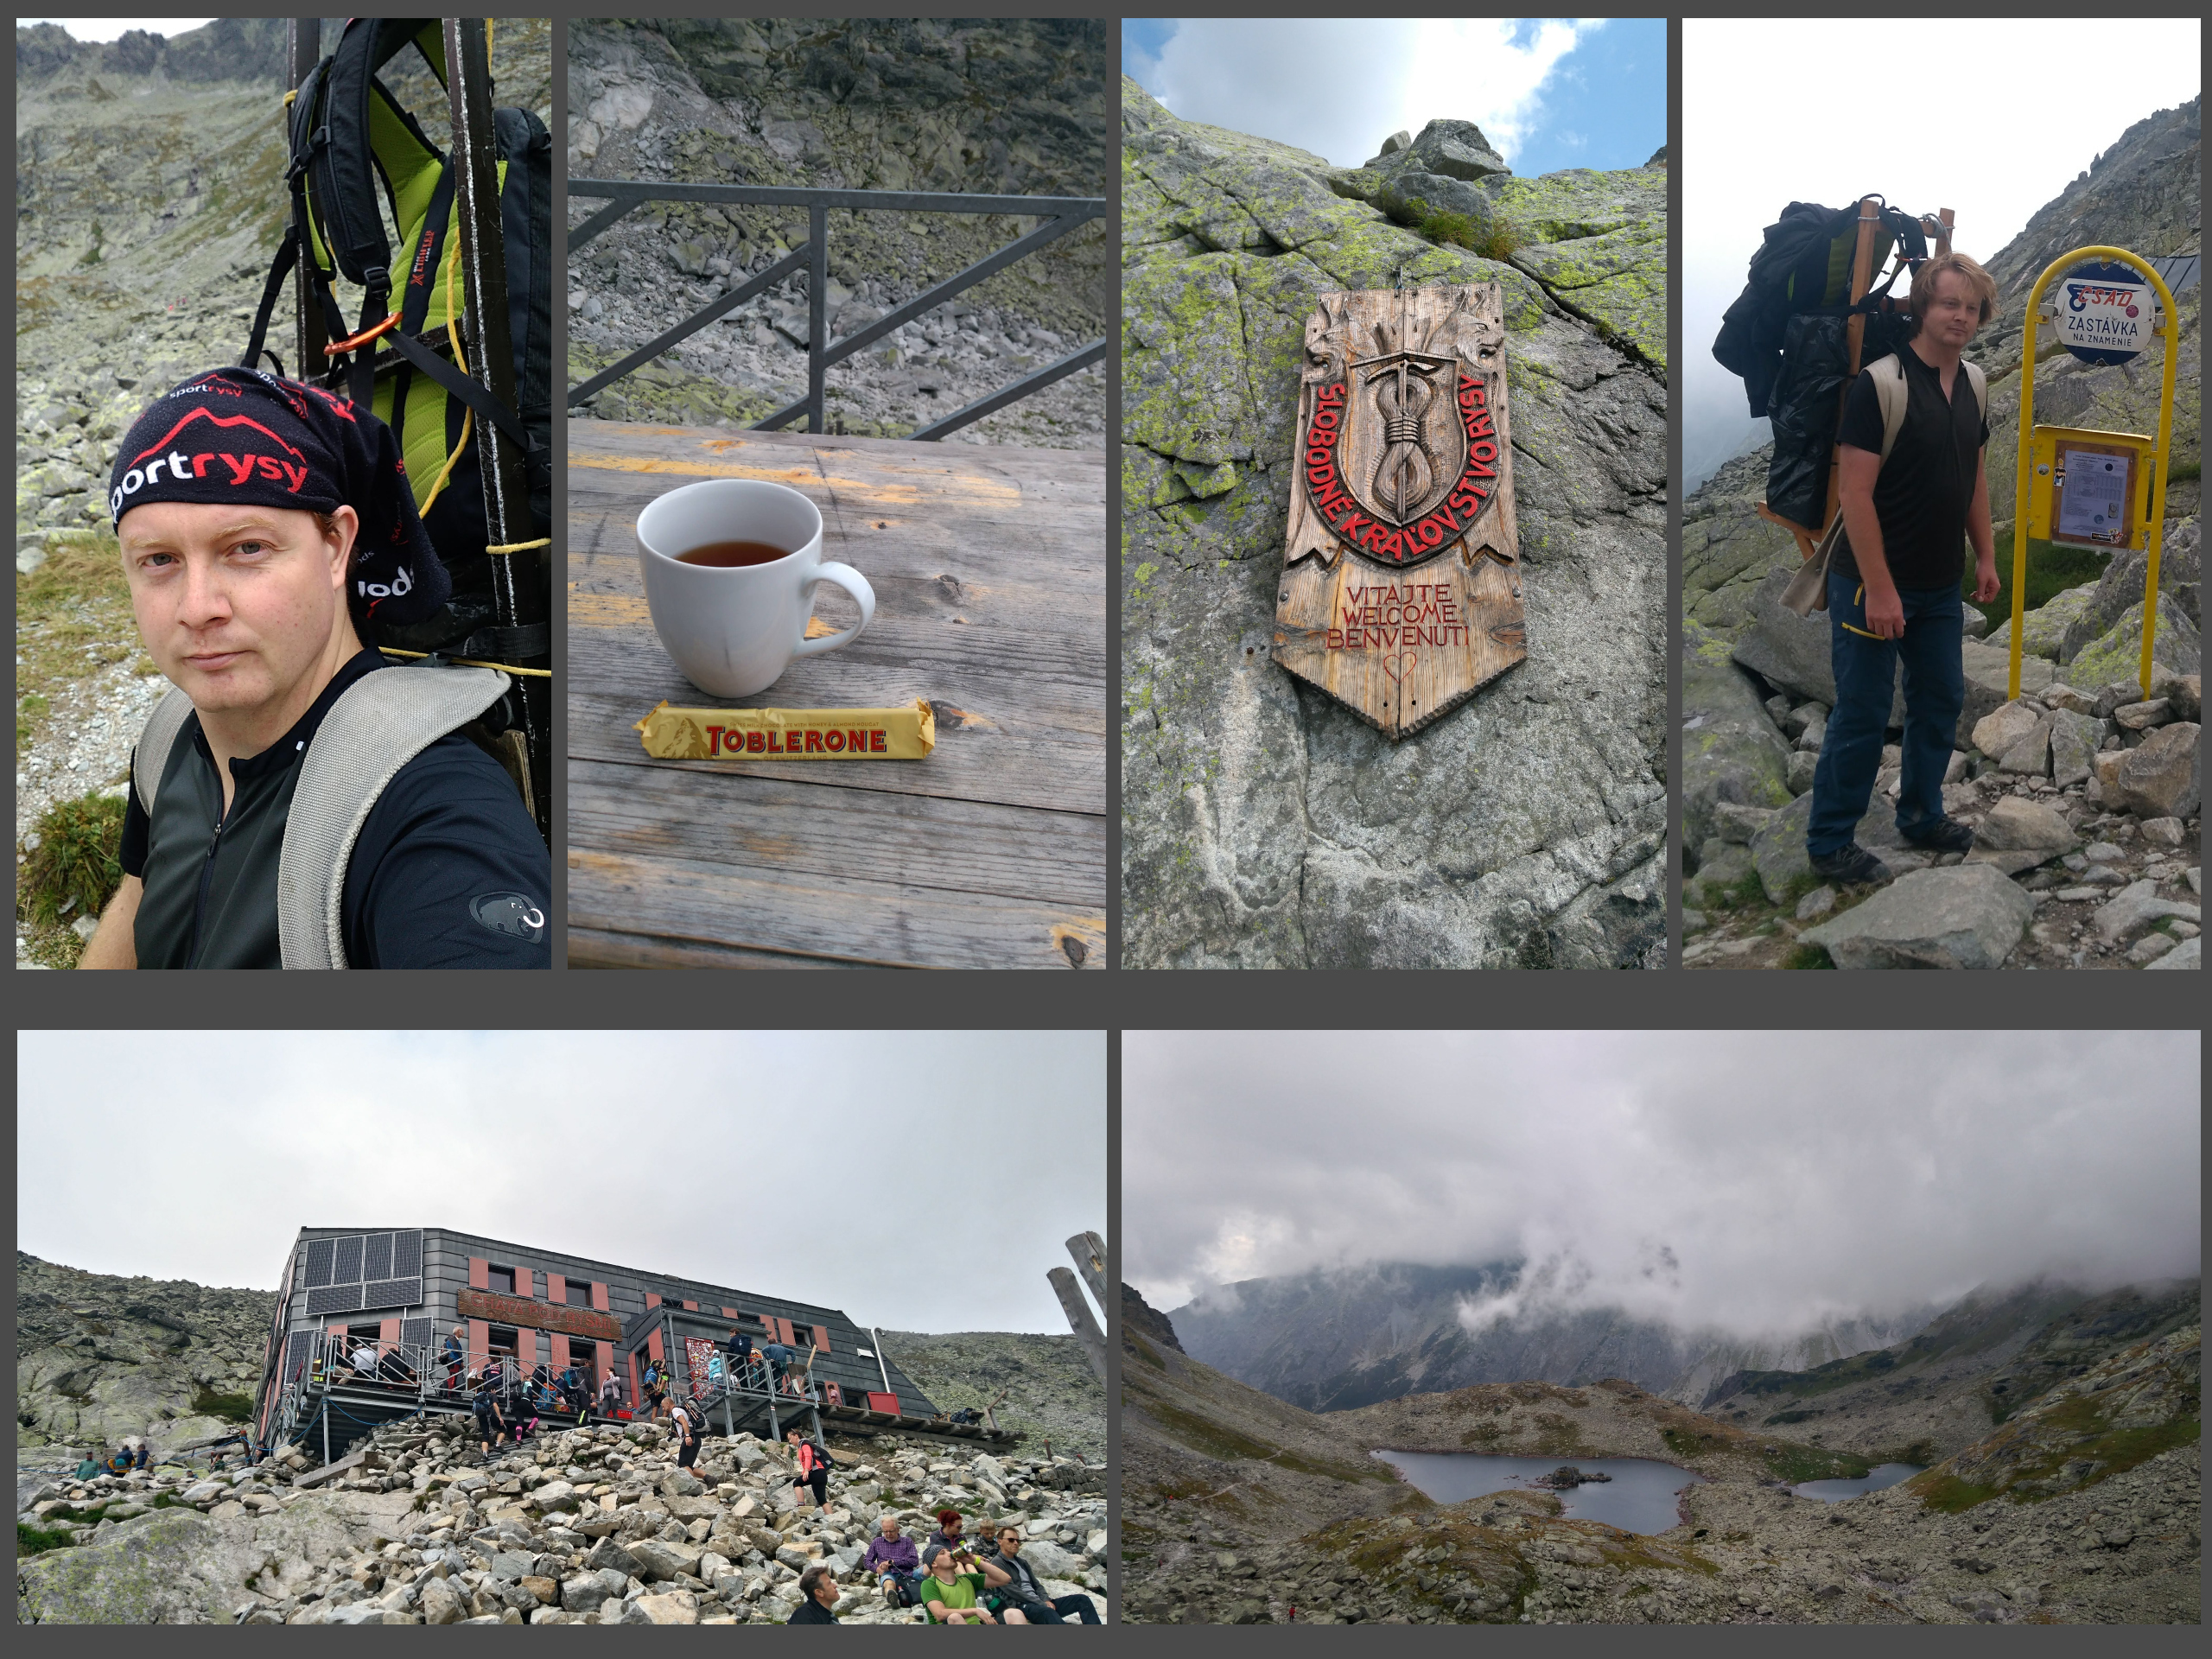
\includegraphics[scale=0.5]{./pictures/me_rysy.jpg}
\end{figure}

\end{frame}



\end{document}
